% Created 2025-04-29 Tue 19:35
% Intended LaTeX compiler: pdflatex
\documentclass[11pt]{article}
\usepackage[utf8]{inputenc}
\usepackage[T1]{fontenc}
\usepackage{graphicx}
\usepackage{longtable}
\usepackage{wrapfig}
\usepackage{rotating}
\usepackage[normalem]{ulem}
\usepackage{amsmath}
\usepackage{amssymb}
\usepackage{capt-of}
\usepackage{hyperref}
\usepackage{minted}
\usepackage{graphicx, siunitx}
\graphicspath{ {./images/} }
\author{Hankertrix}
\date{\today}
\title{Thermodynamics Notes}
\hypersetup{
 pdfauthor={Hankertrix},
 pdftitle={Thermodynamics Notes},
 pdfkeywords={},
 pdfsubject={},
 pdfcreator={Emacs 30.1 (Org mode 9.7.11)}, 
 pdflang={English}}
\begin{document}

\maketitle
\setcounter{tocdepth}{2}
\tableofcontents \clearpage\section{Definitions}
\label{sec:orgd579f59}

\subsection{Spontaneous process}
\label{sec:org81d0a13}
A spontaneous process is a process that, once started, proceeds on its own without a continuous external influence.


A spontaneous reaction occurs slowly if it has a high activation energy \(E_a\).
\subsection{State function}
\label{sec:org07bb188}
A state function is a function or property whose value depends only on the present state, or condition, of the system, not on the path used to arrive at that state.
\subsection{Enthalpy change (\(\Delta H\))}
\label{sec:org1a767aa}
Enthalpy change is the heat change in a reaction or process at constant pressure.
\[\Delta H = \Delta E + P \Delta V\]
\subsection{Entropy (\(S\))}
\label{sec:org189cdba}
Entropy is the amount of molecular randomness in a system.
\subsection{Exothermic}
\label{sec:org4efdfa5}
A process is considered exothermic if its \(\Delta H < 0\). In other words, the reaction releases energy.
\subsection{Endothermic}
\label{sec:orga12d26a}
A process is considered endothermic if its \(\Delta H > 0\). In other words, the reaction takes in energy.
\subsection{First law of thermodynamics}
\label{sec:org10fc1de}
The first law of thermodynamics states that in any process, regardless of the process' spontaneity, the total energy of a system and its surroundings is constant.
\subsection{Second law of thermodynamics}
\label{sec:org387fc73}
The second law of thermodynamics states that in any \textbf{spontaneous} process, the total entropy of a system and its surroundings always increases.
\subsection{Third law of thermodynamics}
\label{sec:org78404b1}
The third law of thermodynamics states that the entropy of a perfectly ordered crystalline substance at \(\qty{0}{\unit{K}}\) is zero.
\subsection{Standard molar entropy (\(S^{\circ}\))}
\label{sec:orgb58f311}
The entropy of 1 mole of a pure substance at \(\qty{1}{\unit{atm}}\) pressure and a specified temperature.
\subsection{Thermodynamic standard state}
\label{sec:orgc7e5e81}
The thermodynamic standard state is the most stable form of a substance. The conditions are:
\begin{itemize}
\item Pressure of \(\qty{1}{\unit{atm}}\)
\item Temperature of \(\qty{25}{\unit{\degreeCelsius}}\)
\item Concentration of \(\qty{1}{\unit{M}}\) for all substances in solution
\end{itemize}

\[\Delta G^{\circ} = \Delta H^{\circ} - T \Delta S^{\circ}\]

\newpage
\section{Formulas}
\label{sec:org604cce5}

\subsection{Change in entropy (\(\Delta S\))}
\label{sec:org38dcc20}
\[\Delta S = S_{final} - S_{initial}\]
\subsubsection{Entropy change for a change in state}
\label{sec:orga79676a}
\[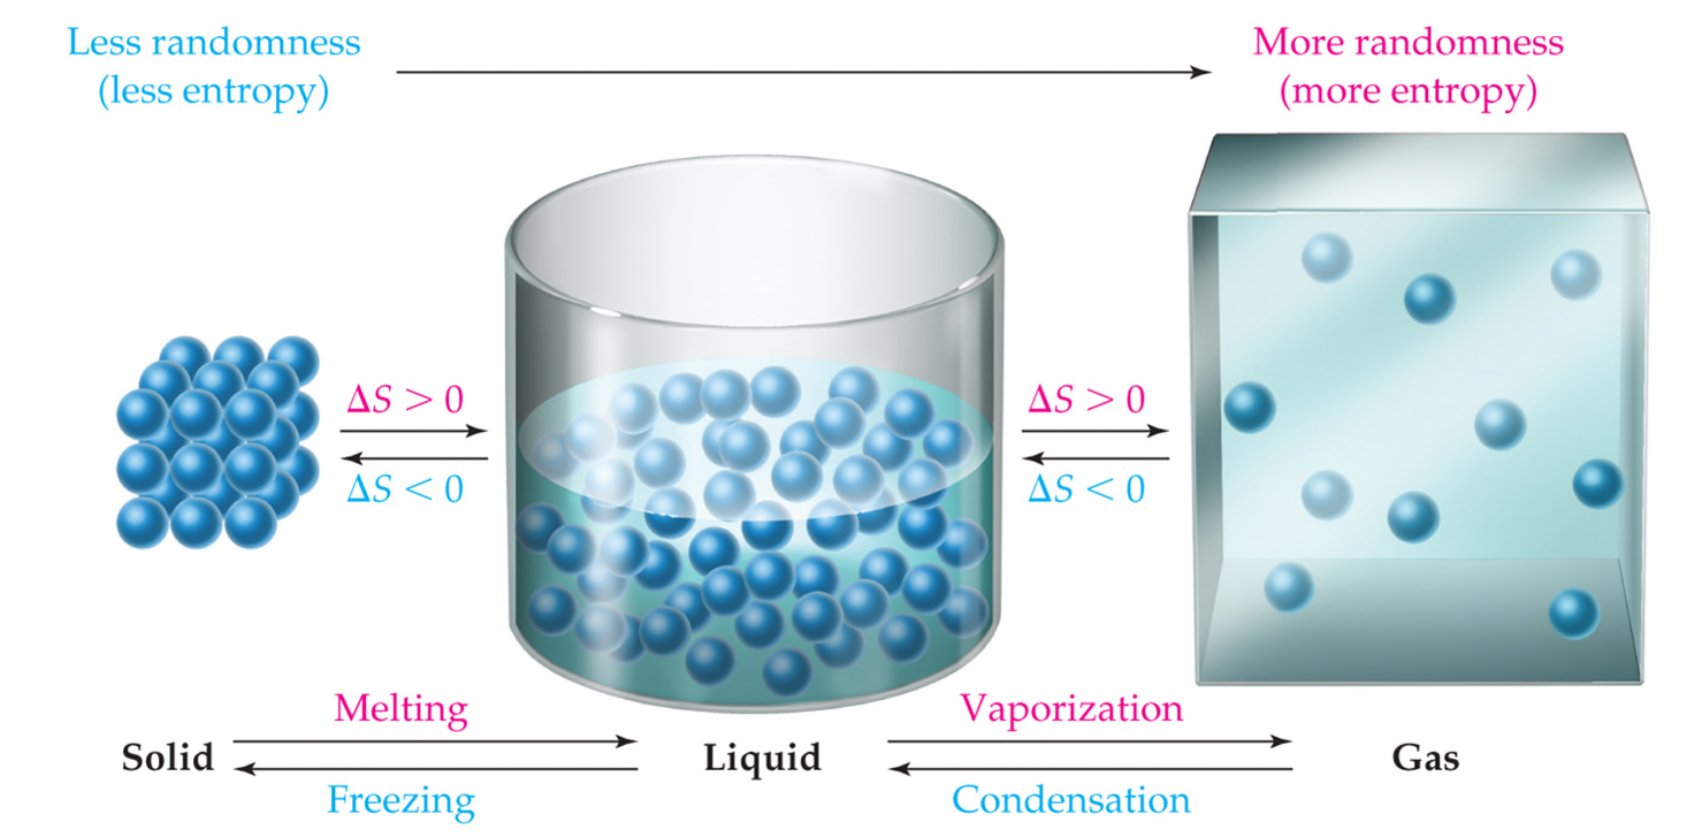
\includegraphics[width = \textwidth]{entropy-change-solid-liquid-gas}\]
\subsubsection{Entropy change for a gas reaction}
\label{sec:org96d2393}
\[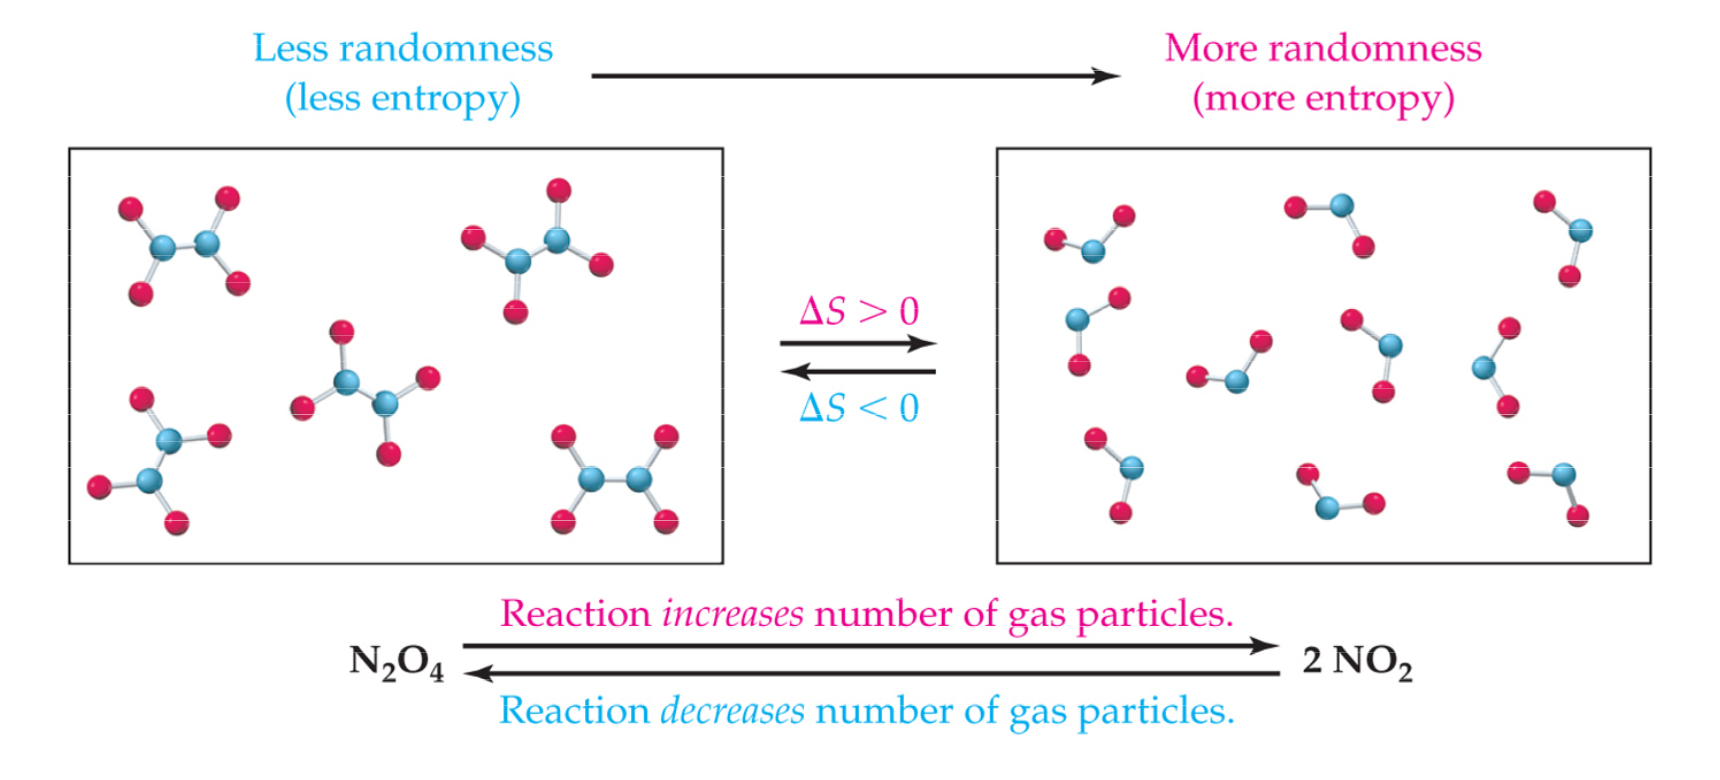
\includegraphics[width = \textwidth]{entropy-change-gas-reaction}\]
\subsubsection{Entropy change for the dissolution of an ionic compound}
\label{sec:orgc4c34cc}
\[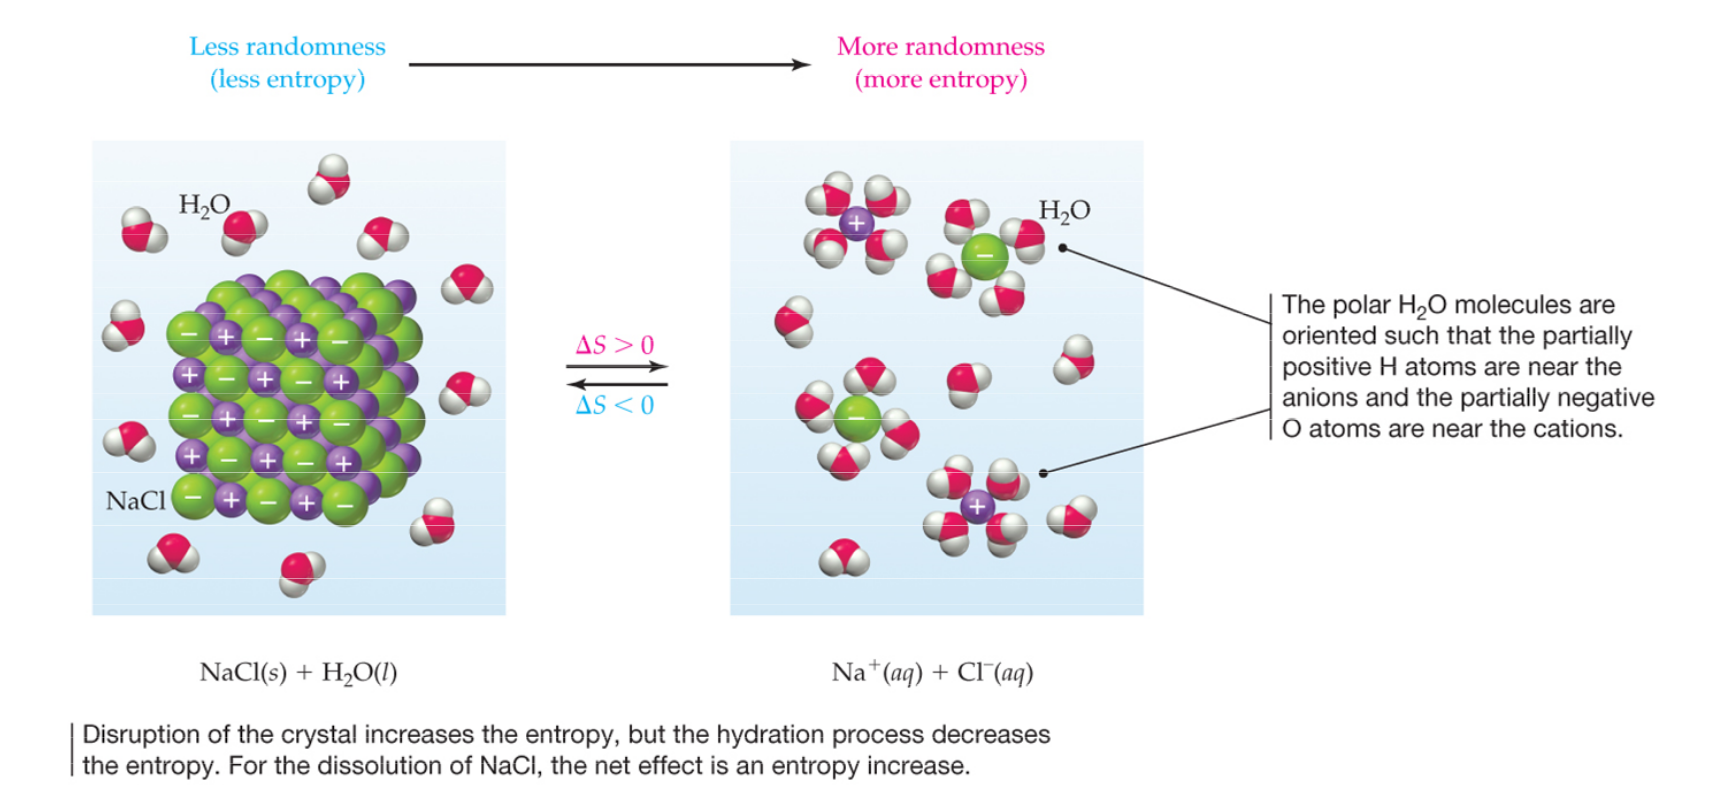
\includegraphics[width = \textwidth]{entropy-change-dissolution-of-nacl}\]
\subsection{Entropy (\(S\))}
\label{sec:org4c16a41}
\[S = k \ln W\]

Where:
\begin{align*}
k &= \text{Boltzmann's constant} \\
&= 1.38 \times 10^{-23} \ \unit{J.K^{-1}}
\end{align*}
\[W = \text{The number of ways that the state can be achieved}\]
\subsubsection{Entropy at various temperatures}
\label{sec:org11d8567}
\[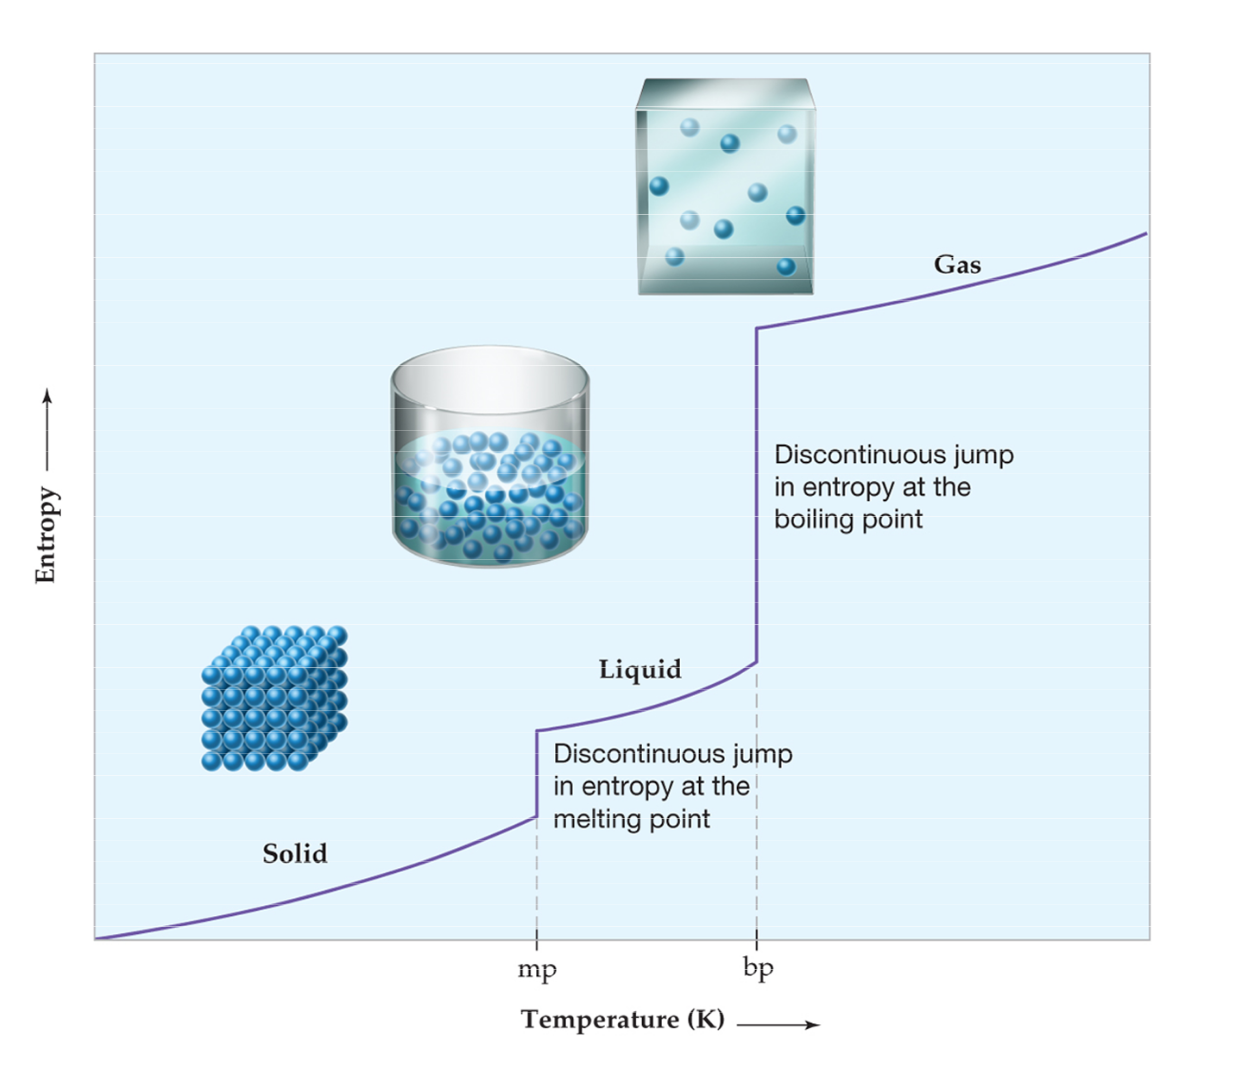
\includegraphics[width = \textwidth]{entropy-vs-temperature-graph}\]
\subsubsection{Entropy at high temperatures}
\label{sec:orgbb1fc9f}
\[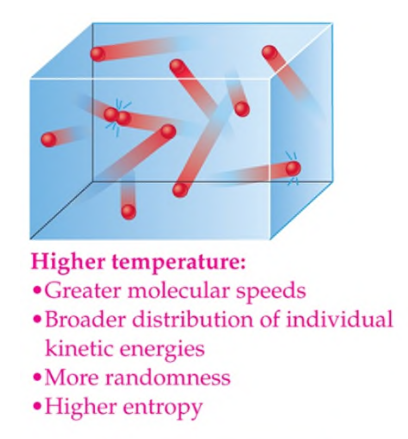
\includegraphics[width = 0.5 \textwidth]{entropy-high-temperature}\]
\subsubsection{Entropy at low temperatures}
\label{sec:org9cfe92b}
\[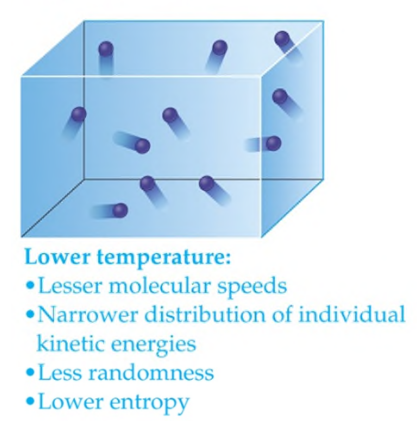
\includegraphics[width = 0.5 \textwidth]{entropy-low-temperature}\]

\newpage
\subsection{Standard molar entropy (\(S^{\circ}\))}
\label{sec:orgddac0cc}
\[\Delta S^{\circ} = S^{\circ}(\text{Products}) - S^{\circ}(\text{Reactants})\]

\[aA + bB \rightarrow cC + dD\]
\[\Delta S^{\circ} = \underbrace{[cS^{\circ}(C) + dS^{\circ}(D)]}_{\text{Products}} - \underbrace{[aS^{\circ}(A) + bS^{\circ}(B)]}_{\text{Reactants}}\]
\subsection{Change in entropy and the 2nd law of thermodynamics}
\label{sec:org5a078ac}
\[\Delta S_{total} = \Delta S_{system} + \Delta S_{surroundings}\]
\[\Delta S_{total} = \Delta S_{sys} + \Delta S_{surr}\]

\begin{center}
\begin{tabular}{c c}
\(\Delta S_{total} > 0\) & The reaction is spontaneous. \\
\(\Delta S_{total} < 0\) & The reaction is not spontaneous. \\
\(\Delta S_{total} = 0\) & The reaction mixture is at equilibrium.
\end{tabular}
\end{center}

\[\Delta S_{surr} \propto - \Delta H\]
\[\Delta S_{surr} \propto \frac{1}{T}\]
\[\Delta S_{surr} \propto \frac{- \Delta H}{T}\]

\newpage
\subsection{Free energy (\(G\))}
\label{sec:orgf956dd9}
\[G = H - TS\]
\[\Delta G = \Delta H - T \Delta S\]

\begin{align*}
\Delta S_{total} &= \Delta S_{sys} + \Delta S_{surr} \\
&= \Delta S_{sys} + \frac{- \Delta H}{T} \quad (\because \Delta S_{surr} = \frac{-\Delta H}{T}) \\
&= \Delta S - \frac{\Delta H}{T} \quad (\because \Delta S = \Delta S_{sys})
\end{align*}

Hence:
\[\Delta S = \Delta S_{total} + \frac{\Delta H}{T}\]

Substituting into the formula for the change in Gibbs free energy
\begin{align*}
\Delta G &= \Delta H - T \Delta S \\
&= \Delta H - T \left( \Delta S_{total} + \frac{\Delta H}{T} \right) \\
&= \Delta H - T \Delta S_{total} + \Delta H \\
&= - T \Delta S_{total}
\end{align*}

Using the second law of thermodynamics and \(\Delta G = - T \Delta S_{total}\):
\begin{center}
\begin{tabular}{c c}
\(\Delta G > 0\) & The reaction is spontaneous. \\
\(\Delta G < 0\) & The reaction is not spontaneous. \\
\(\Delta G = 0\) & The reaction mixture is at equilibrium.
\end{tabular}
\end{center}
\subsection{Standard free energy of formation}
\label{sec:orgb842e16}
\[\Delta G^{\circ} = \Delta G^{\circ}_f (\text{Products}) - \Delta G^{\circ}_f (\text{Reactants})\]

\[aA + bB \rightarrow cC + dD\]
\[\Delta G^{\circ} = \underbrace{[cG^{\circ}_f(C) + dG^{\circ}_f(D)]}_{\text{Products}} - \underbrace{[aG^{\circ}_f(A) + bG^{\circ}_f(B)]}_{\text{Reactants}}\]
\subsection{Free energy changes under non-standard conditions}
\label{sec:orgd231725}
\[\Delta G = \Delta G^{\circ} + RT \ln Q\]

Where \(\Delta G\) is the free energy change under non-standard conditions.


For example, the Haber synthesis of ammonia:
\[N_2 (g) + 3H_2 (g) \rightleftharpoons 2NH_3 (g)\]
\[Q_p = \frac{\left( P_{NH_3} \right)^2}{\left( P_{N_2} \right)^2 \left( P_{H_2} \right)^3}\]
\subsection{Free energy and chemical equilibrium}
\label{sec:org886653e}
\[\Delta G = \Delta G^{\circ} + RT \ln Q\]

When the reaction mixture is mostly \textbf{reactants}:
\[Q << 1\]
\[RT \ln Q << 0\]
\[\Delta G < 0\]

The total free energy decreases as the reaction proceeds spontaneously in the \textbf{forward} direction.


When the reaction mixture is mostly \textbf{products}:
\[Q >> 1\]
\[RT \ln Q >> 0\]
\[\Delta G > 0\]

The total free energy decreases as the reaction proceeds spontaneously in the \textbf{reverse} direction.


\[\Delta G = \Delta G^{\circ} + RT \ln Q\]

At equilibrium, \(\Delta G = 0\) and \(Q = K\):
\[\Delta G^{\circ} = - RT \ln K\]

\newpage
\subsubsection{A diagram to explain the relationship between free energy and chemical equilibrium}
\label{sec:org6358c44}
\[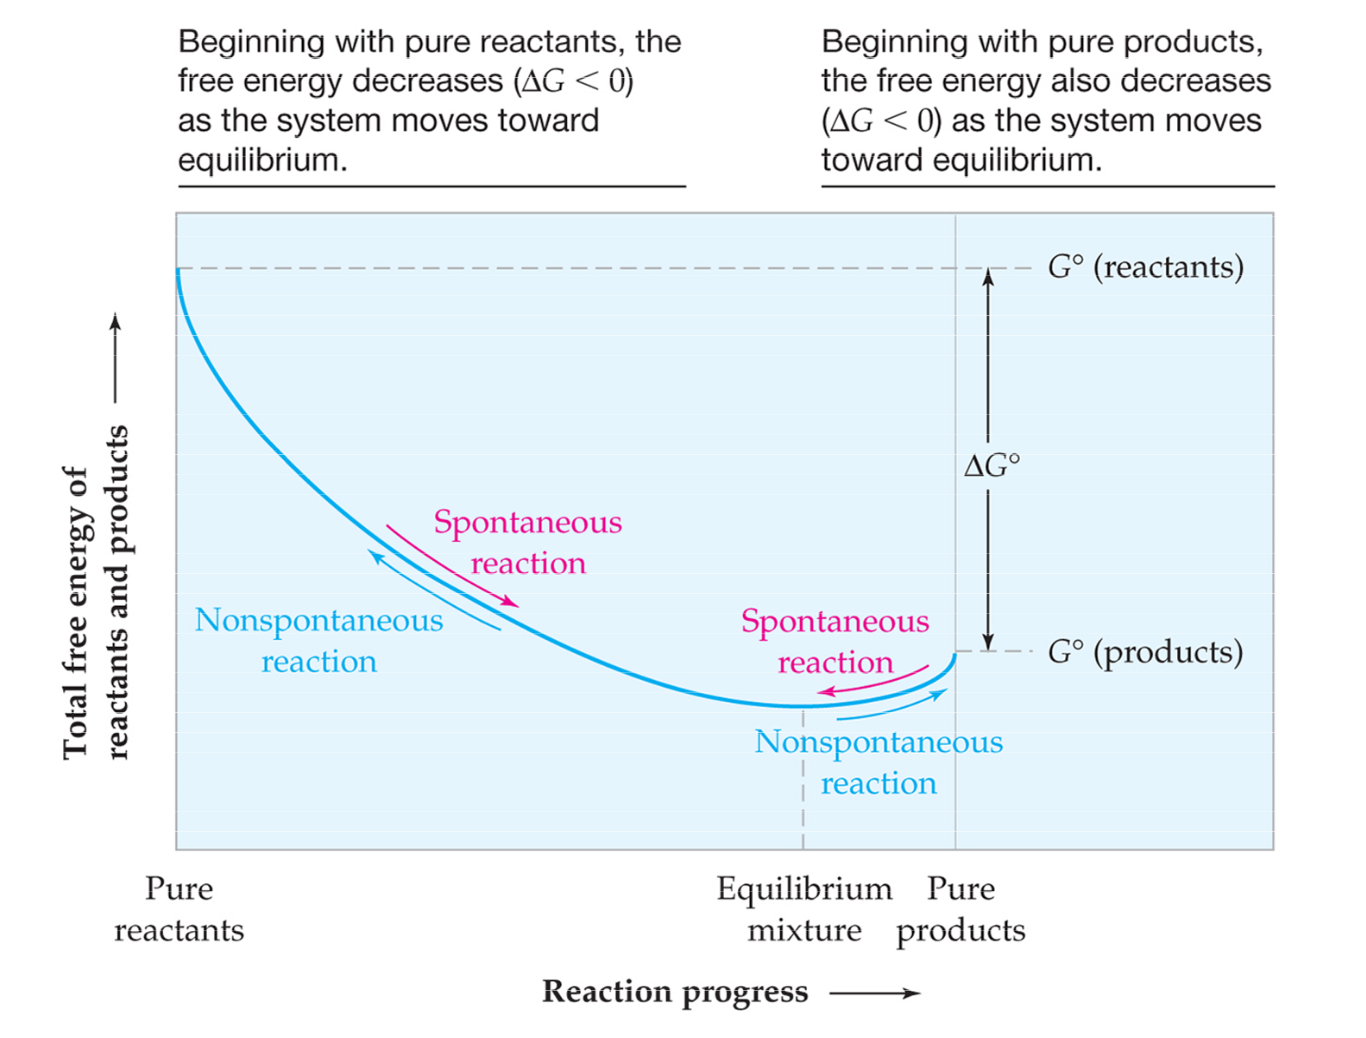
\includegraphics[width = \textwidth]{free-energy-and-chem-equilibria}\]
\subsubsection{Relationship between the standard free energy change and the equilibrium constant}
\label{sec:org17b3812}

\begin{center}
\begin{tabular}{c|c|c|m{20em}}
\(\boldsymbol{\Delta G^{\circ}}\) & \(\boldsymbol{\ln K}\) & \(\boldsymbol{K}\) & \(\textbf{Comment}\) \\
\hline
\(\Delta G^{\circ} < 0\) & \(\ln K > 0\) & \(K > 1\) & The equilibrium mixture is mainly products. \\
\(\Delta G^{\circ} > 0\) & \(\ln K < 0\) & \(K < 1\) & The equilibrium mixutre is mainly reactants. \\
\(\Delta G^{\circ} = 0\) & \(\ln K = 0\) & \(K = 1\) & The equilibrium mixture contains comparable amounts of reactants and products.
\end{tabular}
\end{center}
\end{document}
